\documentclass[a4paper, 11pt]{article}

\usepackage[italian]{babel}
\usepackage{fullpage}
\usepackage[utf8]{inputenc}
\usepackage{graphicx}

\usepackage{listings}
\usepackage{color}

\definecolor{dkgreen}{rgb}{0,0.6,0}
\definecolor{gray}{rgb}{0.5,0.5,0.5}
\definecolor{mauve}{rgb}{0.58,0,0.82}

\lstset{frame=tb,
  language=HTML,
  aboveskip=3mm,
  belowskip=3mm,
  showstringspaces=false,
  columns=flexible,
  basicstyle=\footnotesize\ttfamily,
  numbers=none,
  numberstyle=\tiny\color{gray},
  keywordstyle=\color{blue},
  commentstyle=\color{dkgreen},
  stringstyle=\color{mauve},
  breaklines=true,
  breakatwhitespace=true,
  tabsize=2,
  extendedchars=\true,
  inputencoding=utf8
}

\begin{document}

\title{Riassunto TecWeb2}
\author{Giacomo Manzoli}
\maketitle

I titoli delle sezioni che iniziano con \textbf{\#} sono argomenti non presenti nel programma d'esame


\pagebreak

\tableofcontents

\pagebreak

\section{Usabilità}

\subsection{Homepage}
L'homepage è la pagina principale del sito, l'equivalente della vetrina di un negozio, è dunque importante che sia chiara e ben fatta.
Idealemente l'homepage dovrebbe rispondere ad una versione modificate delle 6W del giornalismo:
\begin{itemize}
\item \textbf{Where} In che sito sono arrivato? In che parte del sito sono?
\item \textbf{Who} Chi rappresenta il sito? Chi ha scritto il contenuto?
\item \textbf{Why} Perché l'utente dovrebbe restare nel sito?
\item \textbf{When} Quali sono le news? Quanto aggiornato è il contenuto?
\item \textbf{What} Di che cosa parla il sito?
\item \textbf{How} Come si può muovre l'utente nel sito?
\end{itemize}
Rispondere a queste domande in modo efficace e in poco tempo è una cosa cruciale dato che normalmente l'utente medio dedica circa 30 secondi alla homepage, tempo che diminuisce ancora se l'utente ha già visualizzato la pagina un'altra volta.
\\
Quando l'utente passa dalla home ad un'altra pagina non sono più necessari tutti gli assi informativi dal momento che si è creato una sorta di legame tra l'utente e il sito.
Grazie a questo legame l'utente è disposto a passare più tempo in una pagina interna (50 secondi in media).

\subsubsection{I timer}
L'utente medio è impaziente, non dedica tanto tempo ad un sito web. Per valutare se vale la pena coninuare con la naviazione del sito l'utente impiega circa 1 minuto e 50 secondi (\textbf{tempo preliminare}) dopodiché se non è soddisfatto abbandona il sito e con il 90\% di possibilità non tornerà mai più, indipendentemente dalla presenza o meno dei contenuti.
\\
Nel caso l'utente decida di restare, il suo \textbf{tempo complessivo} di permanenza non superà comunque i 4 minuti, allo scadere dei quali se non avrà trovato quello che cercava se ne andrà comunque insoddisfatto. Di conseguenza è cruciale che le informazioni siano facilemente reperibili, una buona norma è non superare mai i 3 click dalla homepage.

\subsubsection{Deep Linking}
Se un utente arriva al sito trammite un motore di ricerca è molto probabile che non passi dalla homepage, perciò è importante che anche le pagine interne del sito rispondano ad alcune delle 6W della homepage.
In particolare l'utente dovrebbe sempre riuscire a sapere chi siamo, come tornare alla home e in che punto è nel sito.
Una pratica comune è l'inserimento delle \textbf{Breadcrumbs}, serie di link che rispecchiano il percorso che l'utente avrebbe dovuto fare per arrivare nella pagina.
Ci sono vari tipi di breadcrumbs:
\begin{itemize}
\item \textbf{Location} indicano dove ci si trova nel sito a partire dalla homepage
\item \textbf{Attribute} indica il percorso logico che ha portato dalla homepage alla pagina corrente, non rispecchia necessariamente quello delle pagine
\item \textbf{Path} indica il cammino fisico che ha fatto l'utente all'interno del sito, è di tipo dinamico e viene visualizzato dalla seconda pagina in poi.
\end{itemize}

\subsection{Problemi di navigazione}
Si verificano quando l'asse informativo \textit{where} non è ben sviluppato, cioè quando l'utente non riesce a capire dove si trova rispetto alla home (\textbf{lost in navigation}).
Per risolvere questi problemi si possono usare le breadcrumbs che funzionano abbastanza bene anche se non mostrano il percoso che ha fatto l'utente all'interno del sito, per questo motivo ai link dovrebbero essere associato un colore diverso se sono già stati visitati dall'utente dimunuendone così lo sforzo computazionale. \\
Un'altra cosa da tenere in considerazione è il \textbf{backtracking}, cioè la continua visita di un sito usando frequentemente la funzinalità di ritorno del browser. Questa funzionalità piace tanto agli utenti al punto che preferiscono premere 7 volte il pulsante del browser per tornare alla home piuttosto che usare un link diretto, questo perché richiede meno sforzo computazionale.\\
Bisogna tenere conto di ciò anche quando si aprono i link su nuove finestre o schede diverse, pratica da evitare assolutamente dato che "rompe" il backtracking. L'utizzo di nuove finestre è anche sconsigliato perché se la nuova finestra finisce in background l'utente può non accorgersene e rimanerne frustatrato.

\subsection{Legge di Jakob}
\begin{quote}
Gli utenti passano la maggior parte del tempo su altri siti.
\end{quote}
Quindi è conveniente attenersi alle convenzioni per agevolare la visita degli utenti.

 


\section{Design}
Ad alto livello l'utente si aspetta che un sito web sia ricco di contenuti interessanti.
Il problema è che perché questi contenuti siano accessibili alla maggior parte degli utenti bisogna avere molti accorgimenti perché, per esempio, leggere un testo sul web è fino a 4 volte più impegnativo.

\subsection{Splash e Log In Page}
\textit{problemi non persistenti, quelli del capitolo precendete erano persistenti.}
La splash page è la pagina iniziale del sito di benvenuto ed è meno utile dello Splash di un Magikarp, infatti oltre a non piacere agli utenti (80\%) crea una perdita di tempo perché è priva di contenuto e i timer degli utenti continuano a scorrere.\\
Una versione evoluta della Splash Page è la log in page iniziale, ed è ancora peggio.
Per poter visualizzare il contenuto del sito l'utente deve registrarsi e memorizzare il proprio username e password, creando uno sforzo computazionale elevato. \textit{18, 18, 18, 18...}
Ci sono però alcuni casi dove la pagina di registrazione iniziale ha senso, vedi Facebook, però in altri siti come quello delle poste americane non ha senso.\\
NB: questo ragionamento non comprende le pagine di registrazione per zone specifiche del sito.

\subsection{Scrolling e Layout fisso}
Agli utenti non piace scrollare. Solo il 25\% scrolla nella homepage mentre il 40\% scrolla nelle pagina interne e, in ogni caso, scrollano per circa la dimensione di una pagina, questo perché lo scroll richiede sforzo computazionale.
Perciò quando si progetta una pagina web bisogna tenerne conto e cercare di mettere le informazioni principali nella parte che sicuramente viene vista dall'utente.\\
Per fare ciò si usava un layout fisso, facile da implementare ma non tiene conto del fatto che gli utenti possono avere schermi di risoluzione diversa e che quindi chi ha uno schermo grande non riesce a vedere le informazioni perché sono rappresentate troppo piccole, mentre chi ha uno schermo più piccolo per vedere che la pagina deve scrollare orizzontalmente.\\
Lo scroll orizzontale non dovrebbe mai verificarsi dato che gli utenti non sono abbiutati a questo tipo di scroll e c'è il rischio che l'informazione nascosta non sia mai visualizzata.
Se si sceglie di progettare un layout fisso la taglia di riferimento dovrebbe essere 1024x768

\subsection{Bloated Design}
Certi siti vengono creati con un design troppo spinto che magari piace a chi li progetta ma che crea grande confusione agli utenti del sito.
Alcune caratteristiche tipiche del Bloated Design sono i link lampeggianti e il testo che scorre, ma il non plus ultra è l'audio che parte in automatico all'apertura della pagina e che non è disattivabile.\\
Una possibile conseguenza di questo design sono delle \textbf{metafore visive errate}, vengono cioè rappresentati degli oggetti che sembrano avere una determinata funzinalità ma che in realtà, o non produco nessuna azione oppure producone un'azione che tradisce le aspettative dell'utente, ad esempio un bottone non cliccabile, del testo con lo stesso aspetto di un link o un menù fatto di sole immagini.

\subsection{Plug In, Flash e Video}
I plug in, per quanto utili possono essere, soffrono di due grandi problemi:
\begin{itemize}
\item \textbf{Non sono standard} perciò devono essere scaricati ed installati, l'utente deve quindi fare fatica e perdere tempo.
\item \textbf{Trust Issue:} l'utente medio non sa bene cos'è un plug in e cosa fa, di conseguenza per installarlo deve conoscere bene il sito, altrimenti non si fida.
\end{itemize}
Per questi due motivi il 90\% degli utenti non installa plug in aggiuntivi e abbandona il sito.
Un plug in particolare è \textbf{Flash}, data la sua diffusione è probabile che sia già installato nel computer però si porta dietro altri problemi dovuti ai tempi di caricamento e ad animazioni troppo spinte.
I \textbf{video} invece funzionano decisamente meglio dato che guardare un video richiede poco sforzo da parte dell'utente, vanno però usati con moderazione perché richiedono molta banda per essere scaricati, la lunghezza ideale dovrebbe essere di 1 minuto dato che i timer dell'utente continuano comunque a scorrere.

\subsection{Menù a tendina}
Questa tipologia di menù ha il grande vantaggio che è già nota agli utenti però porta con se vari problemi, primo tra tutti è la chiusura insapettata. Infatti può capitare che l'utente, spostando il mouse da una voce all'altra, esca erronemanete dall'area del menù provocandone la chiusura (54\% delle chiusure sono involontarie), è necesario quindi inserire un timer che lasci aperto il menù per un po' di tempo anche se l'utente esce con il mouse per diminuire le chiusure errate.
Questo timer non deve essere ne troppo corto, sarebbe inutile, ne troppo lungo perché può essere che l'utente voglia veramente uscire dal menù e che la tendina blocchi parte dell'informazione che l'utente voleva visualizzare.
Perché sia efficace un menù non dovrebbe avere più di due sottolivelli, inoltre le voci dovrebbero essere sufficentemente grandi per essere facilmente cliccabili.

\subsection{Testo}
L'idea di base del testo sulle pagine web è che dovrebbe essere leggibile, per ottenere questo risultato sono necesari determinati accorgimenti:
\begin{itemize}
\item la grandezza minima dovrebbe essere di 10pt
\item dovrebbero essere disponibili dei comandi per ridimensionare il testo
\item il font dovrebbe essere unico per tutto il sito, al massimo due font distinti e sarebbero da preferire i font sans-serif come il Verdana
\item il contrasto tra il testo e lo sfondo dovrebbe essere elevato
\item non usare mai immagini al posto del testo
\item evitare l'uppercase che richiede più tempo per essere letto
\end{itemize}
Tendenzialemnte quando si realizza un sito prima si pensa al design e poi al contenuto non considerando che l'utente prima di leggere una pagina web fa una scansione rapida della struttura della pagina.
Questo scannig è molto importante e deve essere il più possibile facilitato, ad esempio un intero blocco di testo è lento da scannerizzare e c'è il rischio che venga saltato dall'utente.
Per evitare ciò è importante suddividere il testo in più paragrafi, ognuno con un titolo descrittivo e inserire delle parole chiave evidenziate (massimo 6/7).
Se sono presenti dei link questi dovrebbero avere un testo corto, descrittivo e identificativo ed essere facilmente identificabili, il classico \texttt{Clicca Qui!} è una pessima idea.\\
Bisogna anche assicurarsi che non si verifichi l'\textbf{effetto ghigliottina} cioè che non il testo non venga troncato per motivi di spazio o che non si crei uno scroll interno del paragrafo.

\subsubsection{Liste}
Utilizzare delle liste aiuta notevolemente la scansione e fa percepire all'utente un senso di ordine (soddisfazione +47\%), è importante però che ci siano almeno 4 elementi e che non ce ne siano troppe.
Le liste dovrebbero essere solamente verticali.













\section{E-Commerce}
In un sito e-commerce la cosa più importante è la vicinanza tra il prezzo e il prodotto, infatti agli utenti piace vedere sia il prodotto che il prezzo contemporaneamente.
Quando per vedere il prezzo è necessario cliccare sull'immagine del prodotto o su un link, si crea una situazione di gambling (\textbf{Gambling click}) nella quale l'utente clicca a caso sperando di trovare il prezzo il che fa diminuire il gradimento da parte dell'utente del 40\%.

\subsection{Farsi pubblicità}
Dato che l'utente non dedica molto attenzione alle pubblicità, si ha poco tempo per impressionarlo.
Comunemente per invogliare l'utente viene visualizzato un prezzo volutamente più basso detto \textbf{Fishing price} oppure un prezzo che esclude le tasse doganali e/o le spese di spedizione (\textbf{Net price}).
Il problema di queste tecniche è che sono pensate per la pubblicità classica, dove l'utente vede la pubblcità e associa al negozio il fatto che ha un prezzo vantaggiso dimenticandosi del prezzo preciso, nel web invece il tempo che passa tra quando l'utente vede la pubblicità e visita il negozio è molto più breve e quindi riesce a riconoscere l'inganno del prezzo.\\
Il 90\% degli utenti che se ne accorge abbandona il sito.\\
Una buona idea è quella di visualizzare una stima del prezzo e poi nel carrello mostrare il prezzo corretto compreso di spese di spedizione, inoltre per i siti che offrono qualcosa di gratuito è bene specificarlo, la parola gratis piace agli utenti.

\subsection{La descrizione del prodotto}
Uno degli errori più grandi che possono fare i proprietari dei siti e-commerce è quello di assumere che il prodotto sia già conosciuto da parte dell'utente.
Se l'utente non trova una descrizione del prodotto che lo soddisfa probabilmente andrà a cercarla su un altro sito, il 95\% degli utenti preferisce acquistare nel sito dove trova la descrizione dettagliata ed è persino disposto a pagare fino al 20\% in più.

\subsubsection{Le foto del prodotto}
Se l'utente è interessato a vederle è bene che siano presenti dato che, oltre a rendere il sito più professionale, i timer dell'utente si bloccano mentre le guarda perché la sua attenzione e posta sui dettagli del prodotto e non sulla pagina web.
Tutto questo funziona se la vista dei dettagli è opzionale e avviene nella stessa pagina.
\section{Eyetrack}
Studio realizzato mediante un eyetracker che registra dove guarda l'utente. Questo studio riguarda come gli utenti agiscono durante la fase di scanning, per mostrare i dati sono state usate \textbf{mappe termiche} con colori più caldi per le zone osservate per più tempo da parte degli utenti.
Tra i vari risultati è emerso che l'utente tende a concentrare di più lo sguardo nella parte in alto a sinsitra del sito, per poi spostarsi da sinistra verso destra e una volta finita la parte superiore verso il basso.
Un'altro sorprendete risultato è stato che gli utenti tendono a concentrarsi più sul testo che sulle immagini, questo perché nel web le immagini sono tendenzialmente o di abbellimento o pubblicità.

\subsection{Testo e paragrafi}
Si è osservato che gli utenti tendono a scansionare meglio il testo quando è su una singola colonna ed è diviso in piccoli paragrafi, inoltre il testo scritto in piccolo, purché sia leggibile, tende ad incentivare la lettura mentre il testo scritto più in grande viene solo scansionato. \\
Per quanto riguarda i titoli, più sono corti, più attirano l'attenzione, si è notato anche che gli utenti leggono la parte più a sinistra del \textit{blurb} (sommario) solo se è scritto come il titolo e non ci sono separazioni.	\\
Le keyword all'interno dei paragrafi sono utili per creare degli hot spot che catturano l'attenzione dell'utente, però non basta che siano semplicemente in bold, devono anche essere sottolineate e di dimensione maggiore.

\subsection{Le immagini}
Anche se l'utente preferisce il testo alle immagini, anche queste vengono visualizzate, se si vuole che un'immagine venga visualizzata è bene che sia almeno 210x210 pixel.
Si è notato che gli utenti tendono comunque a cliccare sopra le immagini anche se ciò non provoca nessun effetto.
Ci sono dei casi particolari in cui le immagini rendono meglio del testo, cioè quando c'è da spiegare all'utente un concetto nuovo, meglio ancora se accompagnato da una spiegazione audio, si è però notato anche che se venogno usate immagini, audio e testo l'utente tende ad ignorare il testo.

\subsection{Layout e Navigazione}
Tra i vari layout testati si è notato che la barra di navigazione è stata notata meglio quando è nella parte alta della pagina e che layout più separati facilitano la scansione della pagina mentre layout compatti sono più efficaci quando l'utente deve leggere il contenuto perché diminuiscono lo scrolling.
Sempre riguardo lo scrolling si è notato che gli utenti scrollano parte della pagina ma la scansionano velocemente cercando qualcosa che attiri la loro attenzione.

\subsection{Pubblicità}
Molto spesso gli utenti tendono ad ignorare la pubblicità e qui pochi che ci fanno caso tendono a dedicarci circa 1 secondo.
Si è notato che i posti migliori dove metterele sono in alto a sinistra oppure in mezzo a del contenuto interessante, è importante però che tra la pubblicità e il contenuto non ci siano margini o separatori. \\
Bisogna stare attenti anche a non abusare della pubblciità altrimenti l'utente si stanca prima e la sua voglia di ritornare nel sito diminuisce dell'80\%.\\
Per ottenere il massimo da una pubblicità conviene che sia scritta sotto forma testuale e che sia grande, inoltre aiuta molto il \textbf{Behavioral Advertising} cioè fornire pubblicità basate sulla cronologia dell'utente ,questo tipo di pubblcità è più apprezzato dagli utenti perché riguarda cose che gli interessano (fino a 100 volte più efficace e aumenta la voglia di ritorno).\\
Altre caratteristiche delle pubblicità\textbf{odiate} dalla maggior parte degli utenti sono:
\begin{itemize}
\item suoni che parto in automatico, 79\%
\item lampeggiamenti vari, 87\%
\item occupano gran parte dello schermo, 90\%
\item si spostano sullo schermo, 92\%
\item non chiare, 92\%
\item coprono il contenuto, 93\%
\item non si possono chiudere, 93\%
\item cercano di farsi cliccare, 94\%
\item si caricano lentamente, 94\% \begin{quote}
Posso sopportare i video che si devono caricare, posso sopportare le pubblicità, ma quando le pubblicità si devono caricare...
\end{quote}
\item pop up, 95\%
\end{itemize}


\section{Legge di Fitts}
$$ T = a + b\cdot\log_{2}(1 + \frac{D}{W}) $$
Dove:
\begin{itemize}
\item \textbf{T} è il tempo che l'utente impiega a spostare il mouse da un punto ad un altro della pagina
\item \textbf{a} rappresenta il tempo di start/stop dell'utente
\item \textbf{b} è la lentezza del movimento, covelocità
\item \textbf{D} è la distanza da percorrere
\item \textbf{W} è la dimesione della destinazione
\end{itemize}
Questa regola è importantissima perché, oltre ad essere corretta nel 98\% dei casi, ci aiuta molto a capire come si comporta l'utente permettendoci di fare alcune considerazioni riguardo l'usabilità delle varie interfacce grafiche.
Alcune conseguenze sono:
\begin{itemize}
\item Il drag'n'drop è sconsigliabile perché viene eseguito più lentamente e stanca prima l'utente, anche per la tensione muscolare necessaria per fare il movimento.
\item I classici menù a tendina sono visti male dall'utente perché certe volte li chiude per sbaglio seguento il cammino minimo. \\
Si sono creati quindi i menù \textbf{bilanciati} nei quali i sottomenù venogno mostrati centrati. Questo perché il web è uno spazio bidimensionale e di conseguenza conta anche la traiettoria.
\item \textbf{Pie Menù} sono dei menù a torta che vengono visualizzati nel punto in cui si trova il mouse diminuendo notevolemente la distanza che l'utente deve compiere per selezionare una voce. Anche se sono più pratici questi menù hanno dei problemi dovuti al fatto che possono visualizzare poche e semplici informazioni, altrimenti gli spicchi diventerebbero troppo piccoli.
\end{itemize}
Una grande spinta verso nuove interfacce ottimizzate secondo la legge di Fitts viene dal mondo dei videogiochi, mondo nel quale l'usabilità è un fattore chiave e nel quale sono disponibili investimenti più sostanziosi.

\subsection{Target Size Rule}
La taglia dei bottoni dovrebbe essere proporzionale alla loro frequenza di utilizzo, come nella suite Office.\\
Un'applicazione ancora più efficacie è l'utilizzo dei bottoni a bordo schermo o negli angoli, in questo l'utente può andare a "sbattere" contro il bordo senza dover fare lo sforzo di fermarsi. Questo fatto si riscontra anche nella formula di Fitts in quanto si può vedere il bordo come un bottone di dimensione infinita, ne segue anche che un bottone a bordo è di più facile utilizzo rispetto ad uno a pochi pixel dal mouse, questo perché il tempo di start/stop influenza maggiormente il tempo totale.

\section{Ricerca}
Per i siti di grosse dimensioni è fondamentale avere un ottimo tool di ricerca, può fare comodo anche su siti più piccoli perché può essere che l'utente sia arrivato al sito trammite \textbf{deep linking} e che quindi non sappia dove trovare l'informazione.\\
Per avere un tool di ricerca si può usare un motore di ricerca già esistenste in modo che esegua la ricerca solamente in locale, questa soluzione però è limitata dal fatto i motori non indicizzano tutto il sito e che se l'utente è arrivato al sito mediante un motore di ricerca, l'utilizzo dello stesso motore di ricerca per cercare in locale produrrà gli stessi risultati.\\
Inoltre può capitare che l'utente venga reindirizzato verso la SERP del motore, portandolo fuori dal sito.\\
Conviene allora creare un proprio tool locale, che rispetti le aspettative dell'utente, cioè che sia simile a quello dei motori di ricerca, seguendo la filosofia \textbf{less is more} per evitare di conforndere l'utente.

\subsection{Come strutturare la ricerca}
Anzitutto bisogna decidere se offrire una ricerca \textbf{classica} o con \textbf{vincoli}, quella con vincoli piace di più agli utenti perché è più efficace, in ogni caso è buona norma offrire entrambi i tipi di ricerca.
La ricerca con vincoli può essere \textbf{statica}, quando l'utente prima inserisce i dati e poi preme cerca, oppure \textbf{dinamica}, che aggiorna i risultati man mano che l'utente inserisce i dati.\\
Entrambe hanno i propri pro e contro, la ricerca statica crea confusione negli utenti perché associano il pulsante cerca alla ricerca classica mentre la ricerca dinamica richiede più tempo per visualizzare i risultati e un maggior sforzo da parte del server.\\
Conviene quindi usare quella dinamica quando ci sono pochi vincoli in caso contrario è meglio quella statica oppure si può usare una versione ibrida nella quale la ricerca parte in automatico quando sono stati impostati tutti i vincoli mentre è statica se alcuni vincoli non sono settati.

\subsection{Box di ricerca}
La misura ideale del box di ricerca è di 30 caratteri, in questo modo viene accontentato circa il 90\% degli utenti.
Dimensionare correttamente il box è importante perché se è troppo piccolo può verificarsi lo scroll orizzontale e inoltre tende ad influenzare l'utente il quale si sente invitato ad inserire query corte che possono influenzare la qualità dei risultati.

\subsubsection{I risultati}
Per visualizzare i risultati si può usare un griglia o una lista, la griglia sembrerebbe ottimale dato che è più compatta e quindi nello stesso spazio vengono visualizzati più risultati, però l'utente per analizzare i risultati disposti in una griglia tende a seguire un cammino casuale che porta ad una perdita di tempo e ad un maggior sforzo computazionale.
Nel lato pratico vengono quindi usate le liste.

\subsection{404: Title not found}
La funzionalità di ricerca gioca un ruolo importante anche quando l'utente visita un link rotto, infatti in questi casi la soluzione migliore è mostrare all'utente sia il messaggio che spiega l'errore sia il tool di ricerca in modo da offrirgli un piano B.
Altre idee come lasciare l'errore di default oppure reindirizzare alla home creano solo confusione/frustrazione.

\subsection{La ricerca 2.0}
Fornire tool di ricerca elaborati con interfacce stile umanoide fa diminuire del 43\% la soddisfazione dell'utente, questo perché un'interfaccia avanzata ne aumenta notevolmente le aspettative.
Se l'umanoide è più un cartone animato, quindi si vede che è virtuale, l'aspettativa cala e di conseguenza il gradimento sale.\\
Ikea come alternativa alla ricerca classica, fornisce anche una ricerca 2.0 con una interfaccia 2D  fatta in stile cartone animate che abbassa le aspettative dell'utente, aumentandone il gradimento fino al +70\%.




\section{Ranking}

Apparire nella prima pagina dei risultati di una ricerca è una cosa cruciale, il 95\% degli utenti non va oltre e in particolare il 51\% di ferma al primo risultato (al secondo classificato vanno il 16\% dei click, 5\% al terzo e ai restanti l'1\% tranne al 10 che si prende il 2\%).
Il punteggio di una pagina viene influenzato sia dal suo contenuto, sia da come è connessa con le altre pagine.

\subsection{TFIDF: Term Frequency - Inverse Document Frequency}

Viene calcolato per ogni keyword ed è basato sul contenuto della pagina, si calcola come il prodotto di due componenti:
\begin{itemize}
\item \textbf{TF} è la frequenza in percentuale con cui compare la keyword all'iterno della pagina
\item \textbf{IDF} è il logaritmo dell'inverso della frequenza della keyword (usato per non penalizzare eccessivamente le keyword complesse e poco frequenti)
\end{itemize}

\subsubsection{Aumentare il TFIDF}
Per aumentare il TFIDF basta inserire ripetutamente le keyword nella pagina.
Ci sono vari posti dove possono essere lette dai motori di ricerca:
\begin{itemize}
\item \textbf{Body Spam} le keyword vengono semplicemente inserite nel body della pagina HTML, sono visibili dall'utente quindi rovinano il conenuto
\item \textbf{Title Spam} le keyword vengono inserite nei titoli \texttt{<h1>, <h2>, ecc.}, è più vantaggioso dato che i motori di ricerca danno più importanza alle keyword nei titoli, inoltre il contenuto della pagina viene alterato marginalmente
\item \textbf{Meta Spam} le keyword vengono inserite nell'apposito meta tag, dato l'abuso di questa tecnica i motori di ricerca tendono a non considerarle.
\item \textbf{Anchor Spam} le keyword vengono inserite come testo di un link che punta alla pagina target, queste keyword vengono valutate di più dato che dovrebbero contenere un sommario della pagina che puntano. Es: \texttt{<a href=\"target.html\">free great deals, free, cheap</a>}
\item \textbf{URL Spam} le keyword vengono inserite nel URL della pagina. \\ Es: \texttt{http://buy-canon-rebel-t3.example.com} 
\end{itemize}
Generalmente queste tecniche di spamming vengono combinate.
In base a dove sono messe le keyword si hanno varie tecniche di spamming:
\begin{itemize}
\item \textbf{Repetition} determinate keyword vengono ripetute, è facilemente individuabile dai motori di ricerca
\item \textbf{Dumping} vengono inserite tante keyword in modo da rendere la pagina significativa per tante query, funziona bene con termini poco usati
\item \textbf{Weaving} vengono copiati articoli/news dal web nei quali si inseriscono delle keyword.
\item \textbf{Phrase Stitching} si attaccano frasi prese da siti diversi così facendo può essere che la pagina compaia nella SERP quando viene cercata una delle frasi
\item \textbf{Broadening} oltre alla keyword che si vuole spammare si usano anche i sinonimi. In questo modo oltre a coprire un range di keyword più vasto si guadagnano anche punti perchè keyword con lo stesso contesto sono ben viste dai motori di ricerca
\end{itemize}
Queste tecniche però rovinano l'aspetto della pagina, vengono quindi usati dei meccanismi di \textbf{Hiding} per preservare l'aspetto della pagina originale.
\begin{itemize}
\item \textbf{Content Hiding} la parte di testo riguardante le keyword viene resa invisibile usando come colore del testo lo stesso colore dello sfondo oppure usando la regola CSS \texttt{display:none;}.
Per nascondere i link si possono usare come ancora delle immagini trasparenti di 1x1 pixel.
\item \textbf{Redirection} una volta caricata la pagina con le keyword si reindirizza l'utente verso la pagina vera. Questo può essere fatto sia con del codice HTML sia con Javascript, conviene farlo con JS dato che i motori di ricerca fanno più fatica a comprenderlo
\item \textbf{Cloaking} simile al redirect, si basa sulla possibilità di distiunguere uno spider da un utente normale, quando la pagina viene richiesta da uno spider gli si fornisce quella contenete le keyword mentre quando viene richiesta da un utente gli si fornisce quella vera. L'identificazione può avvenire tramite indirizzo IP o con l'user-agent della richiesta HTTP.
\end{itemize}

\subsection{PageRank base}
Viene influenzato da come la pagina è connessa con il web e per questo influisce maggiormente nel calcolo complessivo.
La versione base del PageRank considera la rete come un grafo \textit{G(V,E)} dove i vertici sono le pagine web e gli spigoli sono i link tra le pagine.
Data quindi una pagina \textit{v} il suo PageRank è dato da:
$$ \pi_v = \sum_{(v,w) \in E} \frac{\pi_w}{d_w} $$
con
$$ \pi_v \geq 0 \ \forall v \in E $$ 
$$ \sum_v \pi_v = 1 $$
\begin{center}
$d_w$ numero di link uscenti dalla pagina $w$
\end{center}
Si possono però verificare delle situazioni in cui modificando i link uscenti di una pagina, il PageRank della pagina aumenti se le pagine erano collegate in modo circolare (A$\rightarrow$B, B$\rightarrow$C, C$\rightarrow$A se cambio A$\rightarrow$B in A$\rightarrow$C il PageRank di A aumenta).
Inoltre possono esserci gruppi di pagine isolate che rendono questa formulazione del PageRank non equa.

\subsubsection{PageRank} 
Per limitare il problemi del PageRank base si è presa in considerazione la possibilità di passare da una pagina all'altra anche senza passare per un link, con la formula:
$$ \pi_v = (1-\epsilon) ( \sum_{(v,w) \in E} \frac{\pi_w}{d_w} ) + \frac{\epsilon}{N} $$
dove $ \epsilon $ è la probabilità che si effettui un "teletrasporto" e N è il numero totale di pagine.
Anche questa versione soffre dei problemi del PageRank base però ne è meno vulnerabile dato che il PageRank di una pagina non può mai essere 0.
Da notare che se $\epsilon=0$ si torna al PageRank base e se $\epsilon=1$ ogni pagina ha lo stesso PageRank.

\subsubsection{Aumentare il PageRank}

Aggiungere link in ingresso ad una pagina aumenta sempre il PageRank.
Ci sono varie tecniche:
\begin{itemize}
\item \textbf{Infiltration} ci si infiltra in altri siti per aggiungere InLink verso la propria pagina, per esempio sfruttando delle Wiki o i commenti di un blog
\item \textbf{Honey Pot} si inserisce del contenuto interessante (anche copia-incollato) nella pagina, sperando che altri siti si riferiscano a noi
\item \textbf{Link Exchange} ci si accorda con altri siti per linkarsi reciprocamente
\item \textbf{Ressurrection} si compra un dominio scaduto recentemente e si crea una pagina con un link al nostro sito, in questo modo se il dominio aveva dei link entrati questi aumenteranno il PageRank del nostro sito
\end{itemize}

\subsubsection{Spam Farm}
Una spam farm è una struttura di pagine creata con lo scopo di aumentare il PageRank di una pagina target.
Si è dimostrato che, perché una spam farm sia ottima devono valere le seguenti condizioni:
\begin{itemize}
\item Tutte le \textit{boosting pages} abbiamo link uscenti solamente verso la pagina target
\item Non ci siano link tra le \textit{boosting pages}
\item La pagina target abbia link almeno verso una \textit{boosting page}
\item Tutti i link \textit{hijacked} siano verso la pagina Target
\end{itemize}
Il terzo punto è particolarmente importante perché se le \textit{boosting pages} non vengono raggiunte dallo spider dei motori di ricerca non contribuiscono ad aumentare il PageRank della pagina target (\textbf{Reachability}).

\begin{figure}
\centering
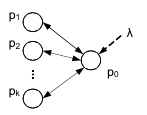
\includegraphics{images/spamfarm_ottima.png}
\caption{Spam Farm Ottima}\label{fig:1}
\end{figure}
Più spam farm possono anche avere link tra loro creano delle \textbf{Spam Farm Alliance}, queste alleanze possono essere di due tipi:
\begin{itemize}
\item \textbf{Alleanze Profonde} le boosting pages di tutte le spam farm dell'alleanza puntano a tutte le pagine target presenti nell'alleanza, se l'alleanza è composta da due spam farm il PageRank delle pagine target diventa la media del PageRank che avevano in precedenza
\item \textbf{Alleanze Superiori} le pagine target dell'alleanza sono tra loro linkate, se l'alleanza è composta solamente da due spam farm il PageRank di entrambe le pagine diventa uguale al massimo dei PageRank precedenti. Le alleanze superiori tra più spam farm possono essere a \textbf{Ring} o \textbf{Complete Core}.
\end{itemize}

\begin{figure}
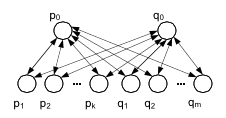
\includegraphics{images/alleanza_profonda.png}
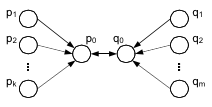
\includegraphics{images/alleanza_sup.png}
\caption{A sinistra: Alleanza Profonda, A destra: Alleanza Superiore}\label{fig:2}
\end{figure}
I motori di ricerca nel tempo hanno adottato delle contro misure, per esempio, per ogni pagina possono calcolare sia il PageRank Base sia quello con "teletrasporto" e calcolarne la differenza (\textbf{Massa di Spam}), se la differenza è notevole analizzano la struttura per vedere se rispecchia la struttura media del web, se trovano una struttura diversa penalizzano il sito (il 95\% dei siti con un'elevata massa di spam sono effettivamente delle spam farm).

\subsubsection{\#Janus Graph}
Il web viene visto come un grafo bipesato, ogni nodo ha un ranking positivo $W+$ e uno negativo $W-$.
La parte positiva viene calcolata con un sistema di ranking qualsiasi, per esempio il PageRank mentre per quella negativa si usa un PageRank basato sull'idea che la parte negativa è duale e opposta: i link vengono "girati" in modo da penalizzare le pagine web che linkano pagine "negative".
$$ R^J = R(G^+) - R((G^R)^-) $$
Per valutare la parte negativa possono anche basarmi su strutture informative già esistenti quali le email.


\section{Semantic Web}
Il Web Semantico è una rete di informazioni collegate tra loro in modo da essere facilemente interpretabili dai computer.
Ogni dato nel web semantico è rappresentato da un \textbf{URI} una stringa composta da due parti \texttt{<scheme>} e \texttt{<path>} che identifica in modo univoco la risorsa.

\subsection{RDF - Resource Description Framework}
RDF è una notazione per modellare informazioni nel web usando una tripa di URI con il seguente significato:
\begin{center}
\texttt{subject property object}
\end{center}
Ogni tripla associa ad un oggetto (\textit{subject}) una proprietà o verbo (\textit{property}) che ha un determinato valore (\textit{object}), un esempio di tripla RDF è dato da:
\begin{center}
\texttt{<http://example.com/rev1> <http://amk.ca/review\#subject> <urn:isbn:1930110111>}
\end{center}
e modella il fatto che la risorsa \texttt{http://example.com/rev1} è relativa all'oggetto \texttt{run:isbn;1930110111}.
I dati RDF possono essere scritti in due formati \textbf{XML RDF} e \textbf{Notation3} entrambi equivalenti, viene preferito Notation3 perché è più semplice e meno verboso di XML RDF.\\ 
Tra i vari vantaggi di Notation3 c'è la possibilità di usare i prefissi:
\begin{lstlisting}
<http://xyz.org/\#subject> <http://xyz.org/\#prop> <http://xyz.org/\#object>
\end{lstlisting}
Può essere scritto in modo più compatto come:
\begin{lstlisting}
@prefix xyz: <http://xyz.org/\#>
xyz:subject xyz:prop xyz:object
\end{lstlisting}
Comunemente sono usati questi prefissi:
\begin{itemize}
\item @prefix : $<$\#$>$ .
\item @prefix rdf: $<$http://www.w3.org/1999/02/22-rdf-syntax-ns\#$>$
\item @prefix rdfs: $<$http://www.w3.org/2000/01/rdf-schema\#$>$ 
\item @prefix dc: $<$http://purl.org/dc/elements/1.1/$>$ .
\item @prefix foaf: $<$http://xmlns.com/foaf/0.1/$>$ .
\end{itemize}
\texttt{dc} e \texttt{foaf} sono dei vocabolari per RDF contenenti delle proprietà e classi usate per descrivere documenti e persone, questi vocabolari sono identificati da un URL in modo da garantirne l'unicità nel web.

\subsubsection{Grafi}
Le informazioni date da un modello RDF possono essere aggretate in un grafo dove i nodi rapresentano le risorse o delle costanti e gli archi rappresentano le proprietà.
\begin{figure}
\centering
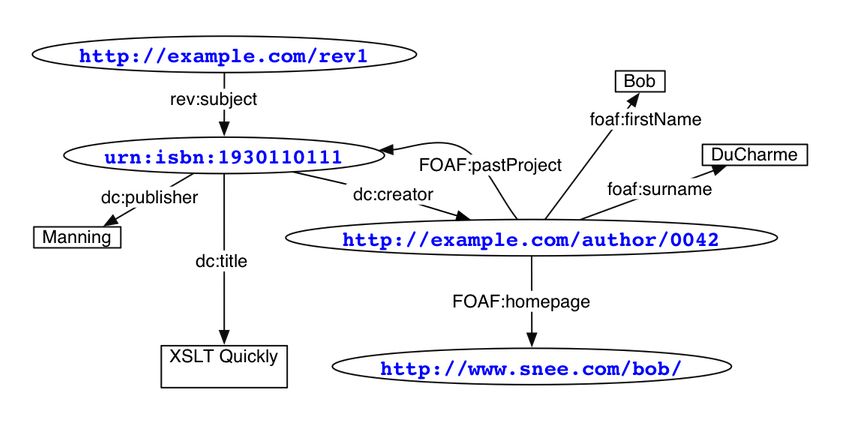
\includegraphics[width=0.8\textwidth]{images/sample_graph.png}
\caption{Esempio di grafo RDF}\label{fig:1}
\end{figure}

\subsection{RDF Schema}
Un RDF-Schema è un vocabolario per RDF che aggiunge sopra a RDF un sistema di tipizzazione, infatti con RDFS è possibile esprimere dei concetti come "Fido è di tipo Cane" e "Cane è sottotipo di Animale".
Ad esempio è possibile definire il vocabolario Pets come:
\begin{lstlisting}
@prefix pets: <http://example.com/xml/pets#> .
pets:Dog rdf:type rdfs:Class .
pets:name rdf:type rdfs:property .

:Fido rdf:type: pets:Dog .
:Fido pets:name "Fido" .
\end{lstlisting}
Oltre a questo RDFS permette anche di definire un dominio e un range di valori per le proprietà:
\begin{lstlisting}
#Impongo che la proprietà nome si possa associare solo a risorse di tipo pets:Dog e che possa avere solo valori di tipo stringa
pets:name rdfs:domanin pets:Dog .
pets:name rdfs:range rdfs:Literal .
pets:name rdfs:comment "Nome del cane" .
\end{lstlisting}
Allo stesso modo è possibile definire una classe come sottoclassi di un'altra:
\begin{lstlisting}
pets:Labrador rdfs:subClassOf pets:Dog
\end{lstlisting}
Grazie a RDF Schema possiamo quindi sapere quali classi esistono e quali proprietà hanno, però non esiste un modo per sapere quando due classi sono equivalenti.

\subsection{OWL - Web Ontology Langueage}
Permette di specificare che relazione c'è tra due oggetti/classi/proprietà appartenenti a vocabolari diversi, ad esempio
\begin{lstlisting}
gen:Person owl:equivalentClass foaf:Person
\end{lstlisting}
Per le proprietà, oltre all'equivalenza, è possibile anche speficare altre informazioni come \texttt{owl:inverseOf}, \texttt{owl:TransitiveProperty} e \texttt{owl:SymmetricProperty}.
Per due risorse è possibile specificare che siano la stessa cosa mediante \texttt{owl:sameAs}.

\subsection{SPARQL}
SPARQL è un linguaggio che permette di scrivere query per lavorare con i dati RDF, offre una sintassi SQL-Like e lavora solamente con RDF e RDFSchema questo garantisce di avere una ricerca che termini sempre, cosa che non sarebbe garantita se usasse OWL.\\
Un esempio di query che ritorna gli url dei blog di "Jon Foobar" è la seguente:
\begin{lstlisting}
PREFIX foaf: <http://xmlns.com/foaf/0.1/>
SELECT ?url
FROM <bloggers.rdf>
WHERE {
	?contributor foaf:name "Jon Foobar"
	?contributor foaf:weblog ?url
}
\end{lstlisting}
\begin{itemize}
\item La prima riga definisce il prefisso per il vocabolario/namespace in uso.
\item La seconda riga definisce che cosa la query deve ritornare, in questo caso la variabile \texttt{?url}. Da notare che in SPARQL le variabili possono iniziare con \texttt{?} o \texttt{\$}
\item la clausola FROM specifica dove eseguire la query, in questo caso è un file locale ma può anche essere un URL
\item Infine la clausola WHERE consiste in una serie di triple che definiscono il pattern da matchare sul grafo
\end{itemize}
\begin{figure}
\centering
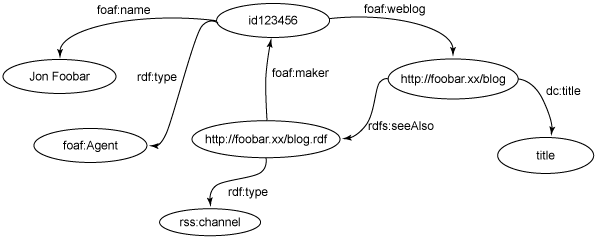
\includegraphics[width=0.8\textwidth]{images/blog_graph.png}
\caption{bloggers.rdf}\label{fig:3}
\end{figure}
Con SPARQL è possibile anche scrivere query molto più complesse sfruttando meccanismi come l'optional matching, l'alternative matching e i filtri che permettono di limitare le variabili, è inoltre possibile lavorare su più grafi contemporaneamente.
Per integrare SPARQL esistono dei framework come \textbf{Jena} che offrono delle API per Java.















\end{document}